\section{Transformer Design}

With given parameters, a transformer is designed and optimized. MATLAB routine for this operation is present in the next section of the report.\\

Remarks and assumptions made in the optimization process are as follows:
\\
\begin{itemize}

\item


\end{itemize}

\begin{figure}[H]
\hspace{1.5cm}
\centering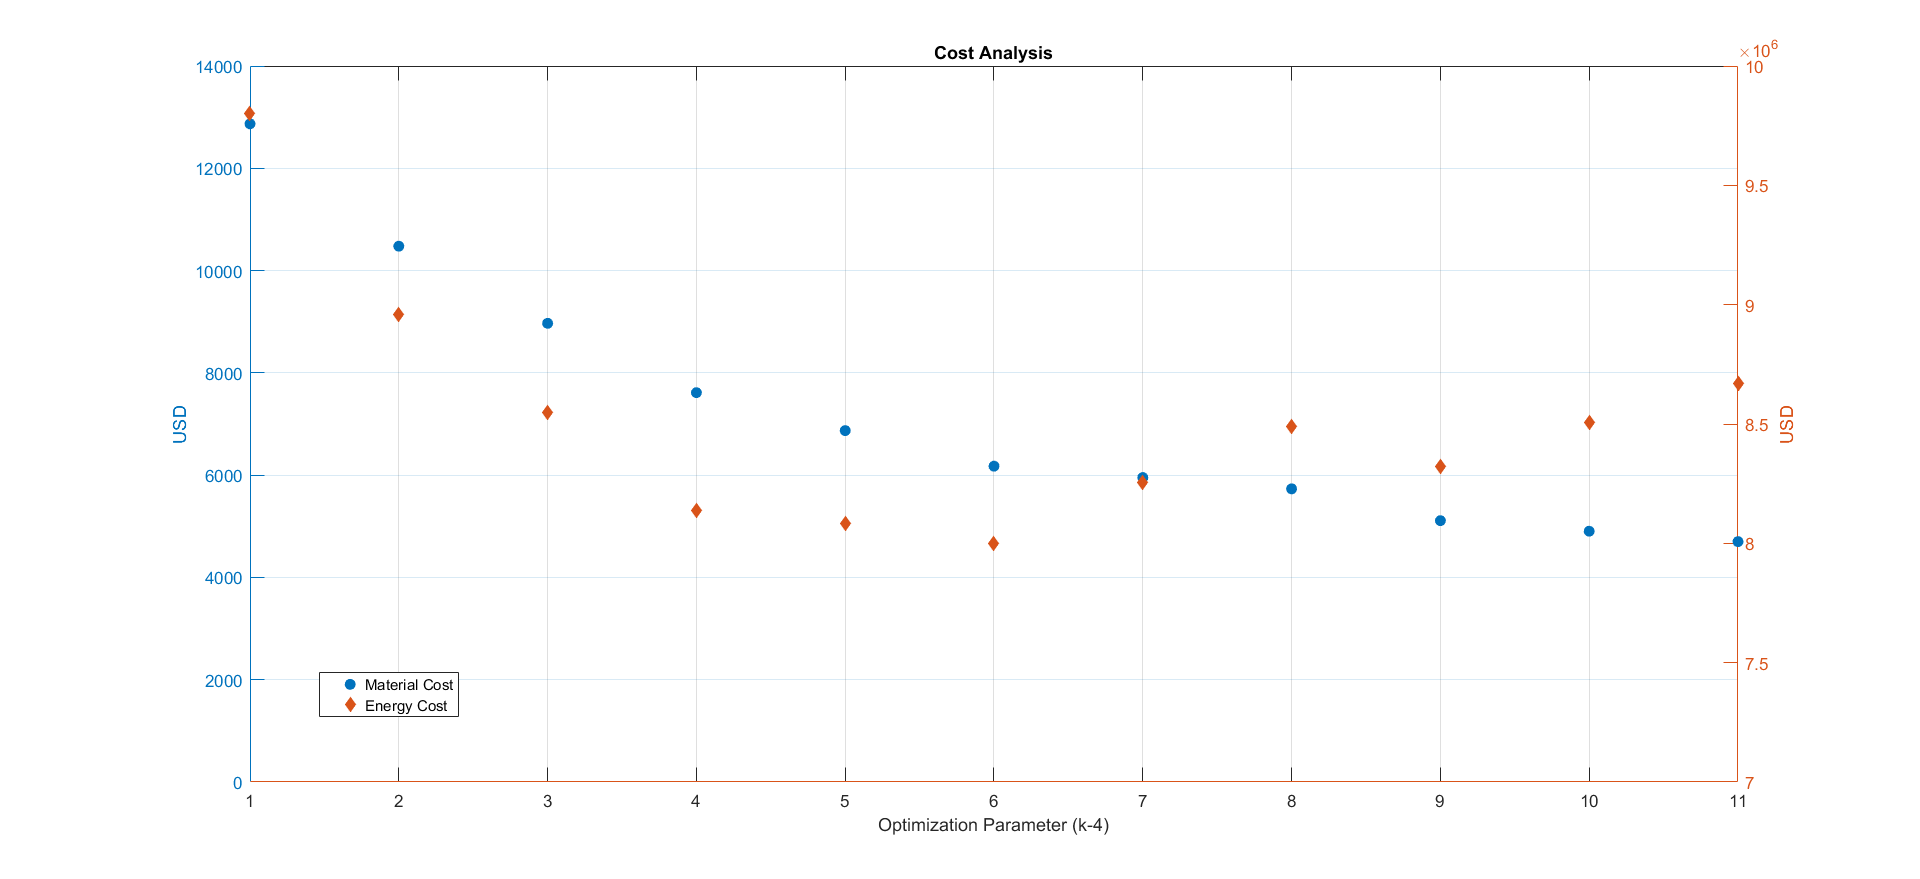
\includegraphics[width=5.5in]{cost.PNG}\\
\caption{Cost Analysis}
\label{cost}
\end{figure} 

\begin{figure}[H]
\hspace{1.5cm}
\centering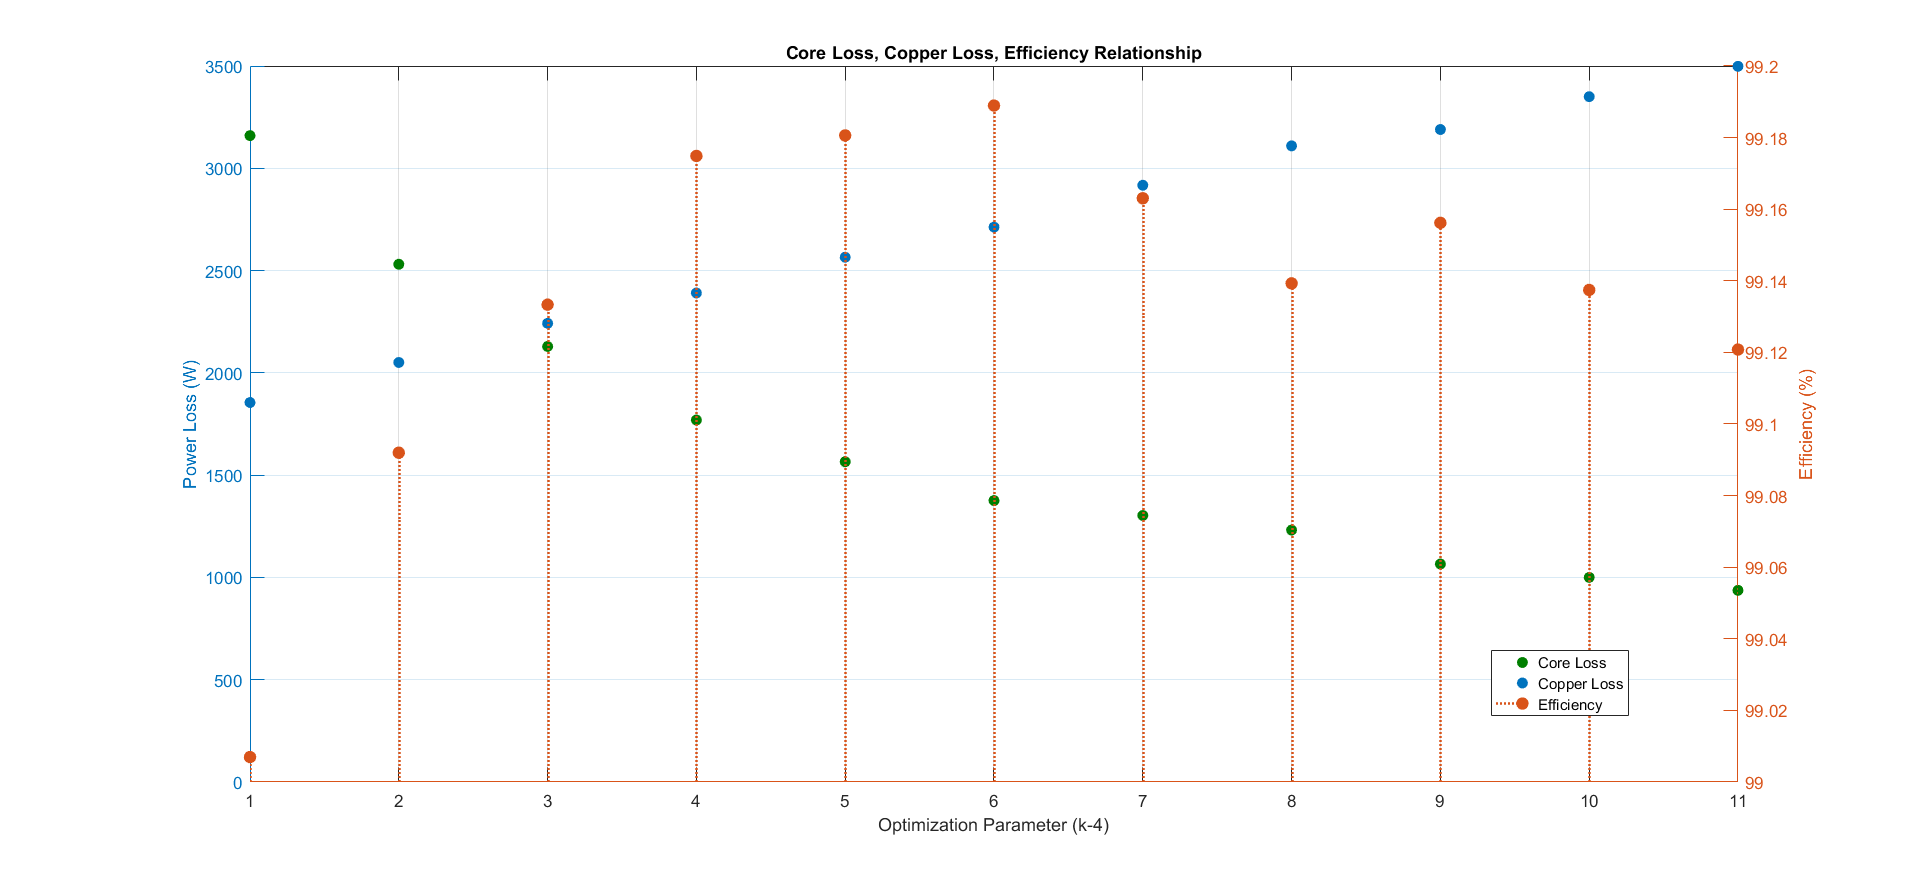
\includegraphics[width=5.5in]{core_copper_eff.PNG}\\
\caption{Relationship Between Core Loss, Copper Loss and Efficiency}
\label{cce}
\end{figure} 

\begin{figure}[H]
\hspace{1.5cm}
\centering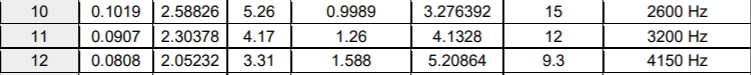
\includegraphics[width=4.5in]{awg.PNG}\\
\caption{Cable Sizes in AWG System}
\label{awg}
\end{figure}

\begin{figure}[H]
\hspace{1.5cm}
\centering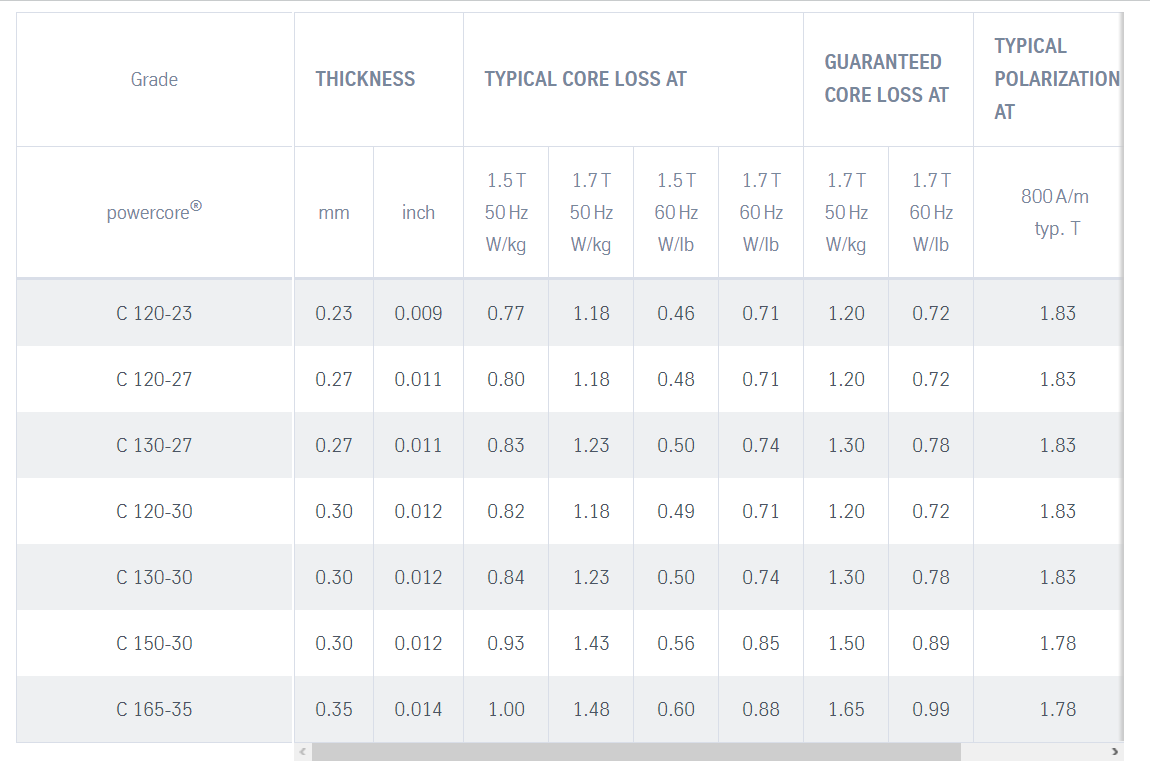
\includegraphics[width=4.5in]{steel_prop.PNG}\\
\caption{Properties of Steel Laminations}
\label{steel}
\end{figure} 
 
